
\section{Objectifs}
\paragraph{}
Lorsque l'on prouve des théorèmes, on a souvent l'impression de faire la même chose, on obtient des reflexes dans de nombreuses situations. Dans les domaines les plus utilisés, il existe maintenant des tactiques résolvant ces opérations répétitives (auto de manière générale, omega pour les entiers naturels, field dans les corps,...).

\paragraph{}
Cependant, lorsque l'on travaille sur des outils plus rares, ou des outils que l'on a soit-même défini, il n'existe pas de tactiques prédéfinies. 

\paragraph{}
Une solution serait de construire soit-même ses propres tactiques lorsque l'on définit de nouveau concept. Malheureusement, celà est difficile. D'une part, parce que Ltac est assez difficile à maîtriser, d'autre part parce qu'il est difficile de transformer un savoir-faire composé de reflexes en une description de ce savoir-faire.

\paragraph{}
L'objectif de ce groupe de travail est de remédier à ce problème. On cherche donc à créer automatiquement, à partir de nombreuses démonstrations, des tactiques permettant de faire des démonstrations similaires.

\section{Les arbres de décisions}

\paragraph{Pourquoi des arbres de décision}
Après une revue des méthodes classiques d'apprentissage, nous avons résolu des théorèmes en coq en analysant à chaque étape notre raisonnement. Nous avons remarqué que nous réflechissions le plus souvent comme des arbres de décision. Nous nous interrogeons sur la structure des hypothèses et du but, à commencer par les noeuds de l'arbre syntaxique de moindre profondeur. La racine du but nous donne assez souvent, à elle seule, la tactique à utiliser. La plupart du temps, si le but est ``T\&U'' on utilise ``split'', si le but est ``forall x, T'' ou ``T -> U'' on utilise intro.  

\paragraph{Définition des arbres de décision}
Un arbre de décision est défini par induction comme étant :
\begin{itemize}
\item Une liste de réponse
\item Une question sur la situation, et pour chaque valeur un arbre de décision
\end{itemize}

\paragraph{Possibilités pour les questions}
D'après ce que nous avons dit plus haut, il est logique de poser les questions sur le haut des arbres. Donc on s'autorise à interroger le noeud à la racine des arbres syntaxiques des hypothèses et du but, ainsi que les fils des arbres déjà interrogés. Les questions qu'on leur pose sont What addr (quel est le token à l'addresse addr?) et Equal addr1 addr2 (est-ce que les tokens à l'addresse addr1 et à l'addresse addr2 sont les même?).


\paragraph{Exemple}
Ici, si le but est de la forme T=T, on répondra $reflexivity$. Son(i,j) désigne le j-ième fils de l'arbre interrogé à la profondeur i.

\paragraph{}
Si la valeur ne correspond à aucune autre, on prend la branche $\$\$OTHER\$\$$
\begin{figure}[h]
  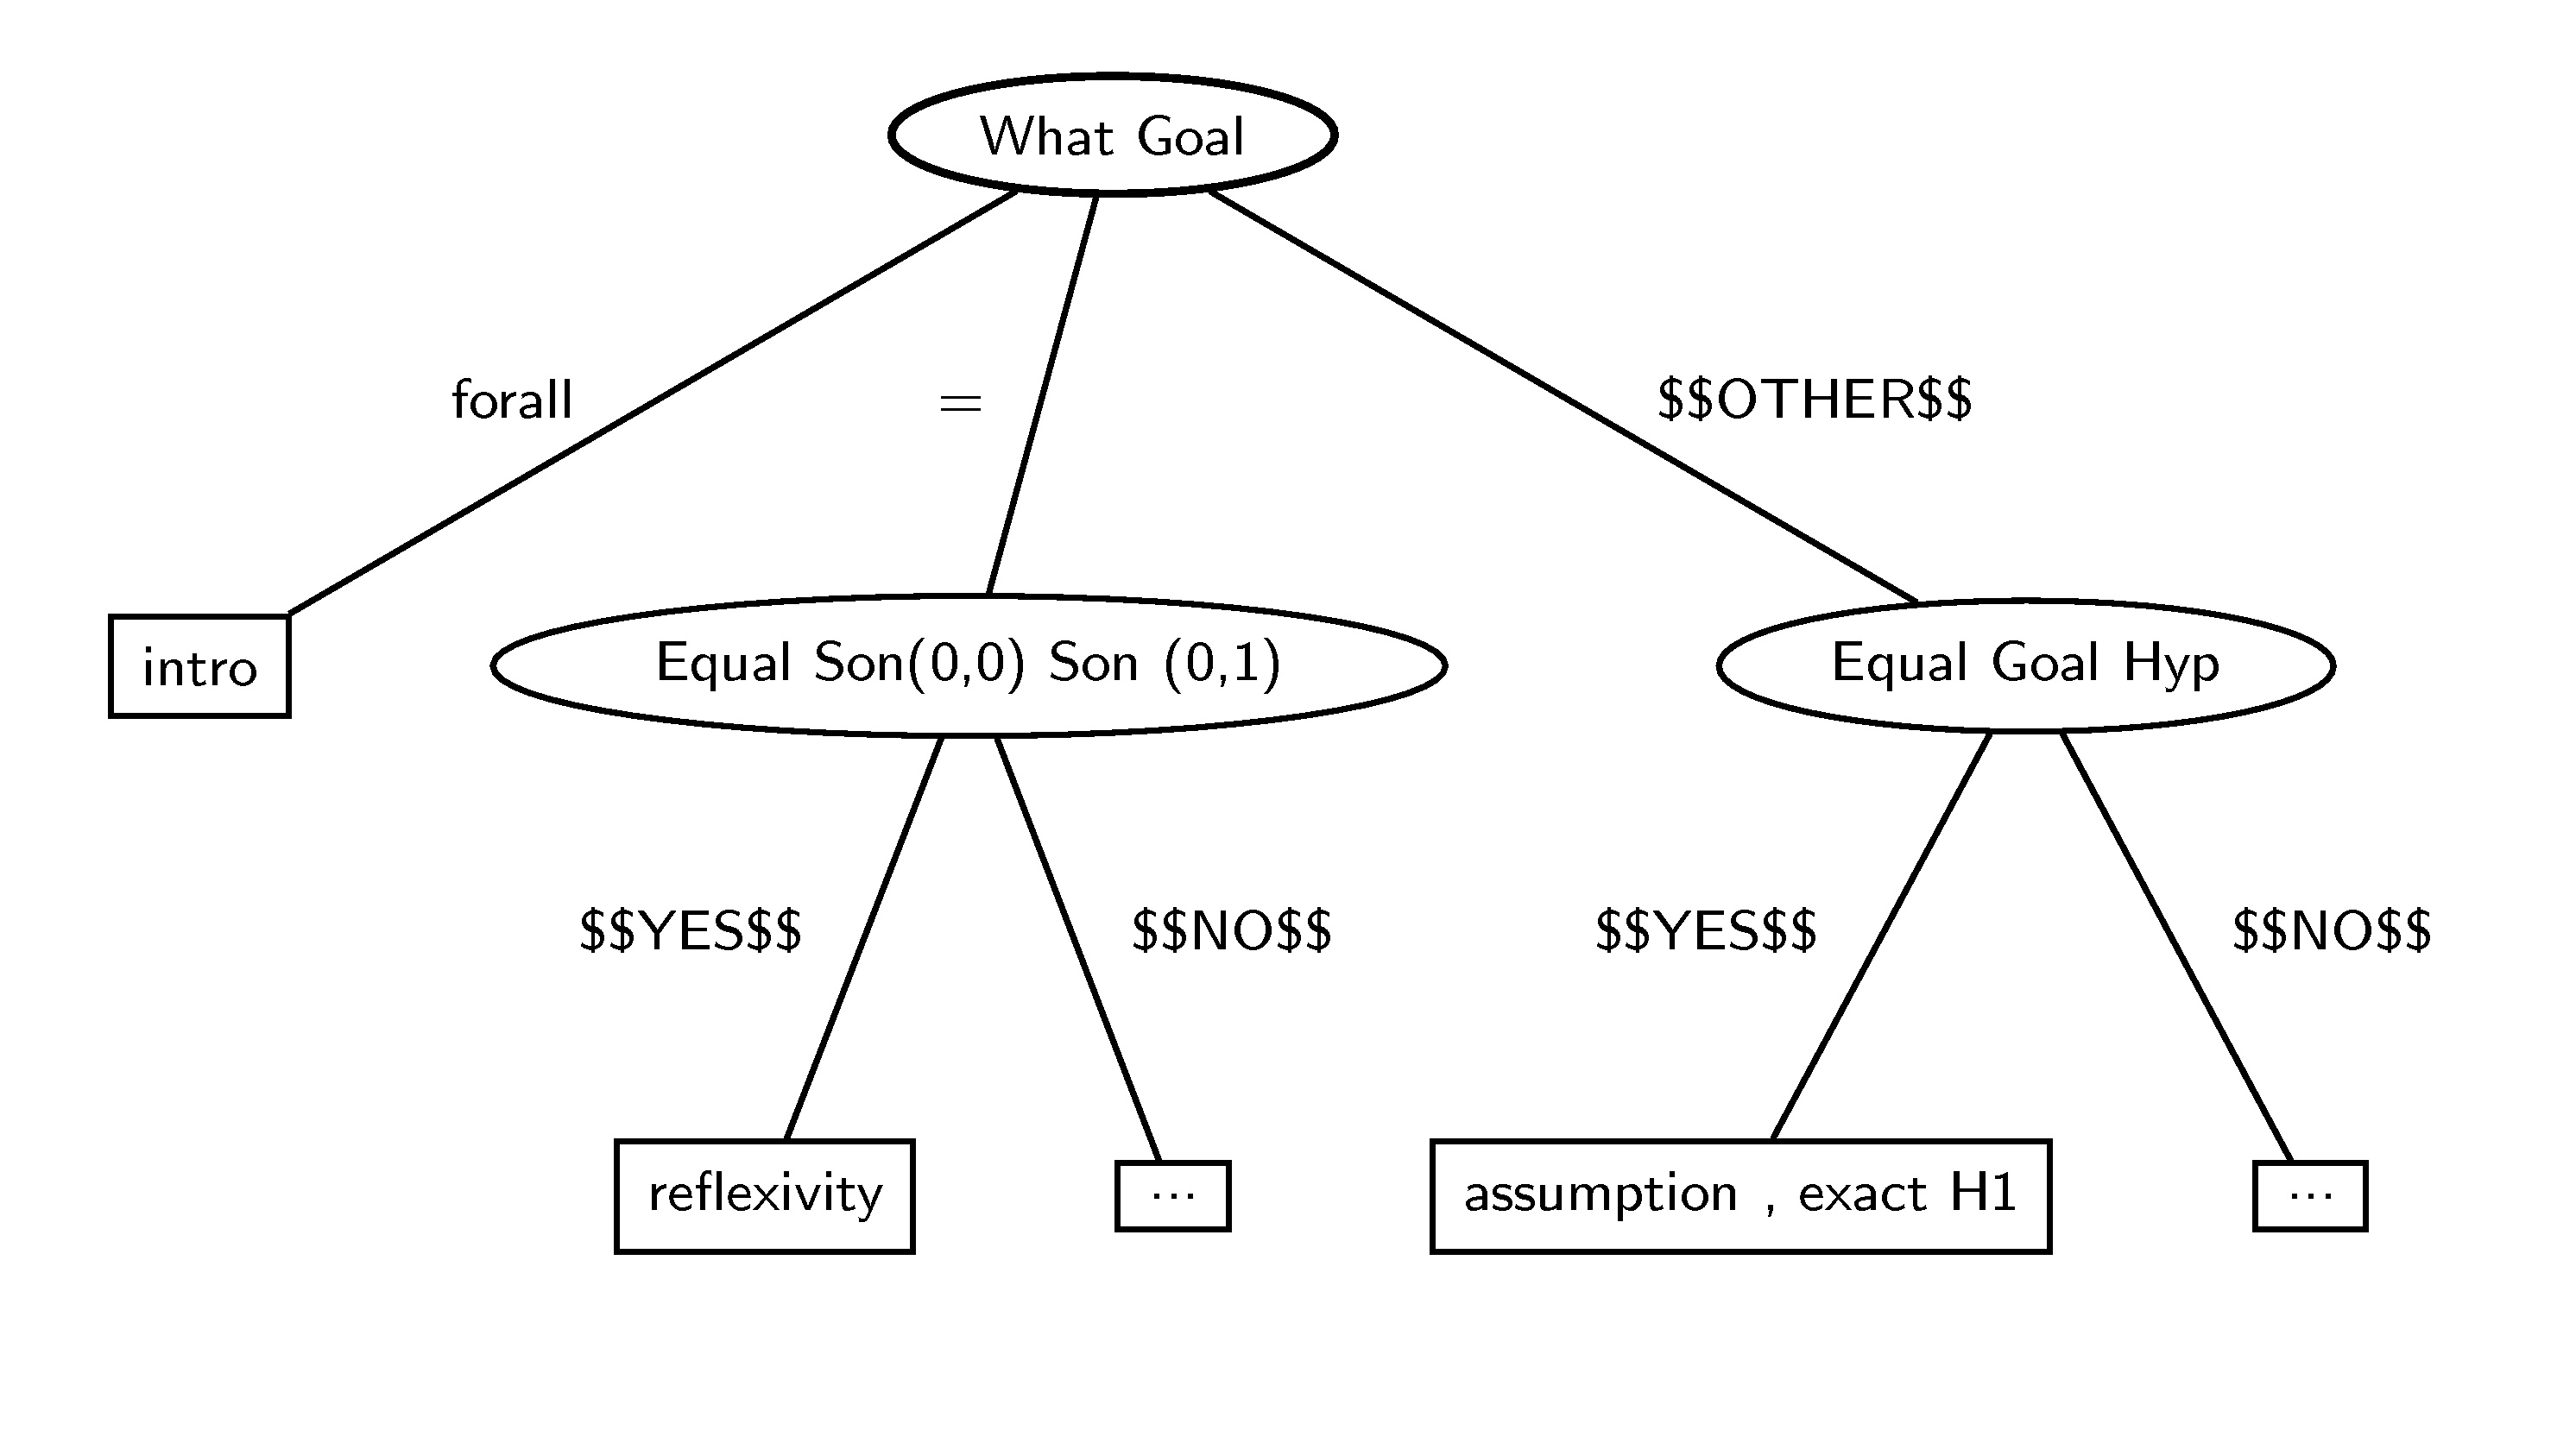
\includegraphics[scale=1.7]{../images/apprentissage/decision_tree.jpg}
\end{figure}


\section{Organisation des modules}
  \begin{figure}[h]
    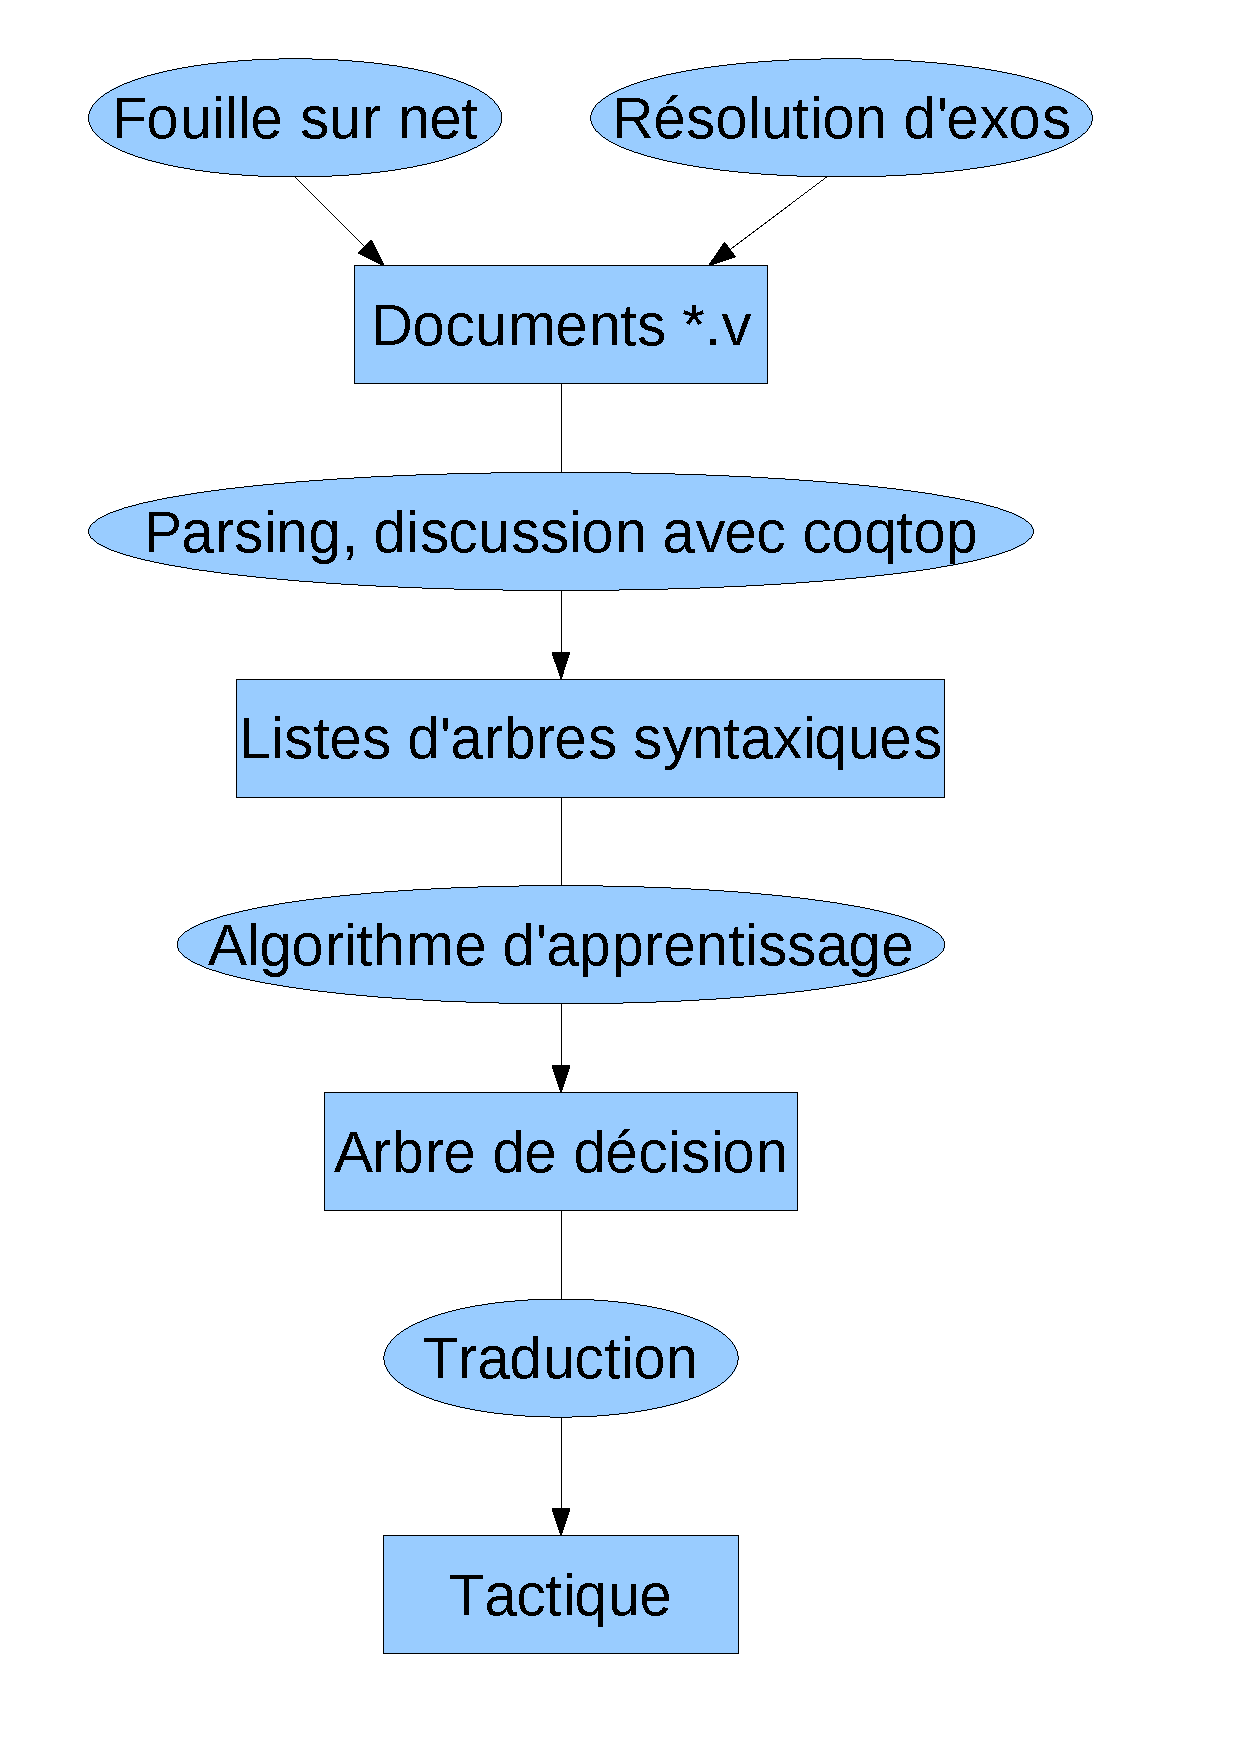
\includegraphics[scale=0.35]{../images/apprentissage/organisation_apprentissage.pdf}
  \end{figure}
  \subsection{Fouille sur net/résolution d'exos}
  Un premier travail est de rassembler un grand nombre de démonstration dans un même domaine. Nous nous sommes essayé sur deux domaines : la logique du premier ordre et les comparaisons d'entiers. Pour des tactiques complète pour ces domaines, il faudrait plus de lignes de démonstrations. Mais ces collections suffisent à tester notre algorithme.
  \subsection{Parsing, discussion avec coqtop}
  Les fichiers que l'on récolte sont des fichiers coqs normaux. Il faut ensuite en extraire les exemples que l'on va apprendre et les mettres sous la forme que l'algorithme d'apprentissage prend en paramètre.

  \subsection{Algorithme d'apprentissage} 
  L'algorithme d'apprentissage transforme ces données experimentales en un arbre de décision.

  \subsection{Traduction}
  L'arbre est transformé automatiquement en une tactique, qui pourra ensuite être utilisée telle quelle.


  \section{Parsing, discussion avec coqtop}
  Pour apprendre à partir d'exemples, il faut exploiter les fichiers de preuves et situer chaque tactique dans son contexte. On voudrait obtenir les réponses existantes au problème « étant données ces hypothèses et ce but, quelle tactique dois-je appliquer ? ». On dispose de fichiers {\tt .v} (vernaculaires) qui correspondent à une liste de tactiques, on veut donc déduire du fichier le contexte dans lequel chaque tactique à été utilisée. On utilise alors coqtop, auquel on donne le fichier {\tt .v} et on stocke les réponses interactives de coqtop dans un fichier ({\tt .out}). Il s'agit effectivement de la méthode d'apprentissage idéale, celle qui se passe du point de vue interactif. Coqtop fournit les hypothèses et le but à prouver à chaque étape, sous forme non formatée car conçue pour l'utilisateur. Les outils pour dialoguer avec coq sont restreints et il n'est pas facile d'obtenir le contexte pour chaque problème de manière directe (problème qui se pose également avec l'IDE). Les formats d'échange XML déjà existant ne permettent pas d'avoir les contextes intermédiaires en cours de preuve. On doit donc analyser la réponse interactive de coqtop, très spécifique. (Il n'est dailleurs pas impossible que cette réponse soit formatée différemment au cours des prochaines versions de coq, mais coqtop a une interface relativement stable car peu utilisée pour son ergonomie). Les analyses lexicales et syntaxiques se font en partie à la main pour le schéma global difficile à appréhender avec des analyseurs classiques de types lex et yacc, car il est nécessaire de prendre en compte espaces, retours à la lignes et tabulations qui ont un sens différent selon la position dans le fichier.
  
  Une autre partie, celle des formules classiques se fait à l'aide d'ocamllex et ocamlyacc, à qui on demande de parser une chaîne de caractères correspondant à une seule formule propositionnelle. On n'utilise une grammaire restreinte à laquelle peuvent s'ajouter au fur et à mesure des jetons spécifiques. Ce n'est un problème que mineur, car l'apprentissage est spécifique à un domaine de problèmes et on peut à la limite adapter la grammaire dans le cas de problèmes utilisant des notations exotiques.

  Il faut aussi analyser les fichier de preuves {\tt .v} pour déterminer les tactiques. Cette analyse est spécifique et on n'a pas besoin d'analyser les fichiers vernaculaires d'une manière si compliquée que celle de coq, qui utilise un nombre important de fichiers de grammaires. Il est important également de prendre en compte les nombreuses tactiques comme {\tt apply (H H2) in H3} qui ne sont pas de simples chaînes de caractères monolithiques (comme {\tt assumption} ou {\tt constructor 2}) et il est pour cela nécessaire de repérer les identifiants dans une chaîne de caractère. Comme coq est très permissif sur les caractères autorisés dans les identifiants il est possible que certains accents ne soient pas pris en compte durant l'apprentissage. (ce qui risque de générer un résultat moins précis à l'apprentissage, mais ne génère pas d'erreur bloquante). Pour les fichiers {\tt .v}, on utilise un système qui combine également l'analyse \textit{ad hoc} et les analyseurs ocamllex/yacc pour le schéma global d'un tel fichier (mais pas pour les termes utilisés dans les tactiques).

\section{Apprentissage}
\subsection*{Entropie}
On considère un ensemble $\{x_i\}_{i \in I}$. On tire au hasard $n$ fois un $x_i$ ($x_j$ est pris avec la probabilité $p_j$). Le meilleur code décrivant la suite des éléments tirés a une espérance de longueur de $n * \sum_{i \in I}{- p_i * \log{p_i}}$. On définit alors l'entropie du tirage comme $ \sum_{i \in I}{- p_i * \log{p_i}}$, soit environ la longueur moyenne du code décrivant quel élément a été tiré. En particulier, on remarque que si une seule réponse est possible l'entropie est nulle.

\subsection*{Application de l'entropie aux arbres de décision}
\paragraph{}Nous voulons qu'à chaque feuille de l'arbre de décision, l'entropie soit minimale. C'est à dire que, pour les exemples conduisant à une même feuille, la tactique à utiliser soit toujours la même. Il faut donc diminuer l'entropie à chaque étape. On veut que l'arbre soit de taille minimale, donc il faut maximiser la perte d'entropie moyenne sur le nombre de noeud total de l'arbre de décision.

\paragraph{}
La maximisation exacte n'est (a priori) même pas dans NP. Il paraît donc préferable d'utiliser une heuristique. A chaque noeud de l'arbre de décision, on cherche à maximiser la perte d'entropie sur le nombre de fils. Pour celà, pour toute les questions possibles, on mesure l'entropie moyenne après la question.

\subsection*{Difficultés surmontées}
Certes, nous nous bason sur un algorithme déjà connu. Mais notre situation est plus compliquée et il a fallu résoudre un certain nombre de problèmes.

\paragraph{Multiplicité des réponses} Un même exemple peut avoir plusieurs réponses à une même question. En effet, si il y a plusieurs hypothèses, il y aura plusieurs réponses à la question \code{What Hypothese?}.
\paragraph{Renumérotation des hypothèses} Lorsque les exemples arrivent à l'algorithme d'apprentissage, la réponse ``apply H0'' sera écrite (``apply \%'' ,[i]) avec i l'indice de H0 dans la liste des hypothèses. Or, ce i ne veut rien dire. Si l'hypothèse H0 avait été à un autre endroit, on aurait quand même appelé H0. Il acquiert du sens seulement si, dans le chemin que l'on fait dans l'arbre de décision pour arriver jusqu'à la réponse ``apply H0'', on pose une question sur une hypothèse et que c'est H0 qui y répond. On représentera alors ``apply H0'' par (``apply \%'', [j]) avec j la profondeur de la question où H0 a répondu. Or il peut y avoir plusieurs hypothèses répondant à la question, on peut se rendre compte plus tard que l'une d'elle n'y répond pas, on peut ne pas encore avoir trouvé de question où H0 répond,...
\paragraph{Grand nombre de réponses} A priori, n'importe quelle fonction ou constante du langage (y compris celles définies par l'utilisateur) peuvent être des réponses. Pour ne pas surcharger l'arbre, dans le cas où seulement certaines réponses sont intéressantes, on a créé la réponse ``\$\$OTHER\$\$'' dans laquelle on met les réponses faisant perdre le moins d'entropie.
\paragraph{Questions non fixes} Le fait d'interroger une question permet ensuite d'interroger ses fils.
\paragraph{Types complexes} Les types des objets sont souvent grand, en témoigne le type 
 \code{(galinaRoot * int * (id*answer) list *(nodeAddress*((galinaRoot* ((id*(int*galinaTerm)) list))list)) list) list} manipulé à plusieurs endroits du programme. Sachant que galinaRoot, galinaTerm, nodeAddress answer sont encore des types composés.
\paragraph{Concepts proches}Il est souvent ardu de s'y retrouver dans les programmes car il y a beaucoup de structures se ressemblant mais qu'il ne faut pas confondre. Par exemple, on peut considérer une hypothèse comme un terme de galina, un token de galina ou une addresse à laquelle on peut poser une question. Il y a les arbres de décision et les arbres syntaxiques. Les réponses à un environnement, les réponses aux questions que l'on pose sur l'environnement. Les tactiques ``élémentaires'' qui sont les réponses dans les exemples d'apprentissage et la tactique qui résultera de l'arbre de décision.

\section{Pipeau?}
L'apprentissage automatique est souvent accusé d'être pipeau. Il y a effectivement une part non négligeable d'approximations et de suppositions dans cet algorithme. Nous allons les lister ici et voir dans quelle mesure elles sont raisonnables.

\subsection*{Supposition de distribution représentative}

\paragraph{}
L'algorithme n'a de sens que si la distribution des tactiques qu'il faut utiliser en fonction des réponses aux questions que l'on peut poser sur l'environnement est la même dans les exemples d'apprentissage et dans les exemples où va être utilisé l'arbre de décision.

\paragraph{}
Les exemples utilisés pour inférer l'arbre et les exemples où l'arbre sera utilisé sont pris dans le même domaine. Donc, d'après la loi des grands nombre, pour un nombre d'exemple suffisament grand la distribution dans les exemples sera aussi proche de la distribution réelle que l'on veut. Le nombre de question est relativement petit, ce qui accélère la convergence. Il y a 2 questions au départ, et dans la pratique il augmente peu. Chaque question posée supprime cette question (sauf les questions sur les hypothèses) et rajoute autant de question qu'il y a de fils. Les arités les plus courantes sont 1 et 2 donc le nombre de questions possible stagne ou augmente de 1 la plupart du temps. De plus, plus le domaine dans lequel nous générons la tactique est restreint, plus cette convergence est accélérée. 

\subsection*{L'arbre n'est pas minimal}
\paragraph{}Pour déterminer les tactiques en minimisant la taille de l'arbre, on utilise une heuristique. Considérons un grand nombre d'exemples. Les buts sont toujours \code{false}. Dans la moitié des exemples, les hypothèses contiennent \code{H:True $\rightarrow$ False}, \code{H':0=0} et des hypothèses aléatoires et la tactique utilisée est \code{apply H}. Dans l'autre moitié, les hypothèses contiennent \code{H:True $\rightarrow$ True}, \code{H':0=1} et des hypothèses aléatoires et la tactique utilisée est\code{inversion H'}. Demander si il y a une hypothèse dont la racine est un \code{=} ou un $\rightarrow$ n'apportera aucune information car tous les exemples ont de telles hypothèses. Donc l'algorithme ne posera pas ces questions là. Donc il n'interrogera jamais les fils droits de H et H' qui sont pourtant les seules informations réellement pertinentes.

\paragraph{} Nous n'avons donc aucune borne d'approximation pour cette heuristique. La seule confiance que nous pouvons lui faire est l'intuition (notre exemple est quand même tiré par les cheveux, l'heuristique semble marcher) et l'expérience.

\subsection*{Choix des questions}
\paragraph{} Il arrive que le raisonnement que fait le mathématicien ne peut pas être traduit dans les termes de l'arbre de décision. Considérons le problème de l'égalité de deux conjonctions: a\&(b\&c)\&(d\&e)=(b\&a)\&(d\&c)\&e. Le mathématiciens va d'abord vérifier que les listes de variables sont les même des deux côtés. Cette question a un caractère global que l'on ne peut pas capturer avec nos questions \code{Equal} et \code{What}.

\paragraph{} Ca semble la limite la plus sévère à notre algorithme. Il faudrait rajouter des questions. Oui mais lesquelles? Si l'on autorise un trop grand nombre de questions par rapport au nombre d'exemples, il y a de forte probabilités pour qu'une question soit considérée comme intéressante alors qu'elle ne l'est pas.

\section{Résultats}

\section{Persepectives}
\paragraph{Compréhension des termes} De même que l'on a réussi à comprendre H dans \code{apply H} comme un argument correspondant à une hypothèse, il faudrait réussir à comprendre \code{cut (z=0)}. Mais ce n'est pas aussi simple. A priori z=0 ne se retrouve nulle part. Ou pas entièrement. On pourrait voir, dans les arbres syntaxiques interrogés, lesquels ont le plus grand sous-arbre commun avec z=0.

\paragraph{Connexion avec l'IDE} Il serait bien que depuis l'IDE, l'utilisateur puisse dire quelle preuves il veut rajouter dans les bases d'exemples pour quels domaines. Les tactiques serait réactualisées régulièrement pour correspondre aux nouveaux exemples.

\paragraph{Bases d'exemples sur le net} Plus il y a de preuves, meilleures seront les tactiques. On peut imaginer de grandes bases de données sur internet. Chaque utilisateur de coquille les utiliserait et les alimenterait.

\paragraph{Update à la volée} Actuellement, si on veut rajouter des exemples il faut refaire entièrement l'arbre. On pourrait chercher un moyen pour actualiser l'arbre de décision avec les nouveaux exemples même si on a effacé les exemples d'avant.

